% !Mode:: "TeX:UTF-8"

%为了便于查找和修改,还可以拆分文件为子章节,并通过input导入。

\chapter{模板结构}

模板文件的结构,如下表所示:
\begin{table}[ht]\centering
\begin{tabular}{r|l|l}
\hline
\multicolumn{2}{l|}{main.tex }       & 主文档,在其中填写正文  \\ \hline
content 文件夹 & abstract.tex         & 中/英文摘要、关键词     \\ \cline{2-3} \hline
content 文件夹 & content.tex          & 正文                     \\ \hline
content 文件夹 & acknowledgements.tex & 致谢                     \\ \hline
content 文件夹 & appendix.tex         & 附录                     \\ \hline
\multicolumn{2}{l|}{figures 文件夹}   & 存放图片文件            \\ \hline
\multicolumn{2}{l|}{codes 文件夹}     & 存放代码                \\ \hline
\multicolumn{2}{l|}{NBUThesis.cls}   & 定义文档格式             \\ \hline
\multicolumn{2}{l|}{refs.bib}        & 参考文献存放             \\ \hline
\multicolumn{2}{l|}{nbuthesis.bst}   & 参考文献格式             \\ \hline
\end{tabular}
\end{table}

无需也不要改变、移动上述文档的位置。

\section{标题风格}
宁波大学各学院本科毕业论文的模板存在一些差异,最明显的是章的标题风格。可以使用“\verb|ZhChapter|”选项切换两种风格:
\begin{itemize}
\item \verb|\documentclass{NBUThesis}|:章标题效果为“\textbf{1~~模板结构}”
\item \verb|\documentclass[ZhChapter]{NBUThesis}|:章标题效果为“\textbf{第一章~~模板结构}”
\end{itemize}

\section{使用步骤}

\begin{enumerate}
\item 进入 content 文件夹, 打开 abstract.tex 并分别填写中、英文摘要、关键词;打开 acknowledgements.tex 填写致谢;打开 content.tex 填写正文部分;打开 appendix.tex 填写附录内容。

\item 将图片放入 figures 文件夹,支持 PDF、JPG、PNG 等格式的图片,最好是 PDF 格式的矢量图。

\item 将参考文献信息录入 refs.bib,并在正文中正确引用。

\item 使用 XeLaTeX 编译。具体见 \ref{sec-compile} 节。
\end{enumerate}

\section{编译方法} \label{sec-compile}

按照 xelatex $\rightarrow$ bibtex $\rightarrow$ xelatex ($\times 2$) 的顺序编译,直接生成~pdf 文件。

% %%%%%%%%%%%%%%%%%%%%%%%%%%%%%%%%%%%%%%%%%%%%%%%%%%%%%%%%%%%%%%%%%%%%%%%%%%%%

\chapter{字体操作}
\section{字体调节}

\begin{tabular}{lllll}
\verb|\songti|    & {\songti 宋体}    &~~~&\verb|\bfseries|          & {\bfseries 粗宋体}\\
\verb|\sffamily|  & {\sffamily 黑体}  &~~~&\verb|\bfseries\sffamily| & {\bfseries\sffamily 粗黑体}\\
\verb|\ttfamily|  & {\ttfamily 楷体}  &~~~&\verb|\bfseries\kaiti|    & {\bfseries\kaiti 粗楷体}\\
%\verb|\itshape|   & {\itshape 斜宋体} &~~~&\verb|\bfseries\itshape|  & {\bfseries\itshape 粗斜宋体}\\
\end{tabular}

\section{字号调节}
%字号命令: \verb|\zihao| \index{zihao}
\begin{tabular}{ll}
\verb|\zihao{0}| &\zihao{0}  初号字 English \\
\verb|\zihao{-0}|&\zihao{-0} 小初号 English \\
\verb|\zihao{1} |&\zihao{1}  一号字 English \\
\verb|\zihao{-1}|&\zihao{-1} 小一号 English \\
\verb|\zihao{2} |&\zihao{2}  二号字 English \\
\verb|\zihao{-2}|&\zihao{-2} 小二号 English \\
\verb|\zihao{3} |&\zihao{3}  三号字 English \\
\verb|\zihao{-3}|&\zihao{-3} 小三号 English \\
\verb|\zihao{4} |&\zihao{4}  四号字 English \\
\verb|\zihao{-4}|&\zihao{-4} 小四号 English \\
\verb|\zihao{5} |&\zihao{5}  五号字 English \\
\verb|\zihao{-5}|&\zihao{-5} 小五号 English \\
\verb|\zihao{6} |&\zihao{6}  六号字 English \\
\verb|\zihao{-6}|&\zihao{-6} 小六号 English \\
\verb|\zihao{7} |&\zihao{7}  七号字 English \\
\verb|\zihao{8} |&\zihao{8}  八号字 English \\
\end{tabular}

% %%%%%%%%%%%%%%%%%%%%%%%%%%%%%%%%%%%%%%%%%%%%%%%%%%%%%%%%%%%%%%%%%%%%%%%%%%%%

\chapter{列表环境}

缘分来了真的挡也挡不住。讲一个真实的故事,2024 年大三,暑假快结束时从北京坐高铁回学校,斜对面坐了一个很乖巧的小女生,眼睛大大的,脸圆圆的,非常可爱,怀里抱着一个小熊书包。我有点无聊,于是玩起了手机上的五子棋小游戏。这个时候女生说话了,说她也喜欢下五子棋,并且很厉害。然后我们一起玩了几局五子棋小游戏,一边玩一边聊天。她刚高考完,马上上大一,安徽人,小我四岁,趁着刚开学前有时间,她爸妈带着她和她弟弟一起去北京玩,去了故宫和八达岭,刚好我也去过,于是聊了很多。

凌晨天快亮的时候我醒了,发现她靠在我肩膀上睡的觉。我先到站,她和她家人还有两站,我想留个联系方式,于是我们加了微信。两天后她给我发来了消息,然后我们互相介绍对方的家乡的样子,发生活照片,说了很多话。后来开学了,我问她是哪个学校的,她说她是宁波大学的。宁波大学,简称“宁大”,位于浙江省宁波市。由浙江省人民政府、宁波市人民政府共同举办的省属普通高等学校。是国家“双一流”建设高校、省部市共建高校、浙江省首批重点建设高校、浙江省高水平大学建设高校、“浙江省国际化特色高校”首批建设单位和宁波市国际人文交流基地。学校于 1986 年由包玉刚捐资创立,并于 1992 年被列入中国高校招生第一批录取院校。1996年,原宁波大学、宁波师范学院和浙江水产学院宁波分院三校合并,组建新的宁波大学。截至 2025 年 3 月,宁波大学设有 23 个学院:
\begin{itemize}
\item 机械工程与力学学院
\item 物理科学与技术学院
\item 数学与统计学院
\item ...
\end{itemize}
拥有 6 家附属医院:
\begin{enumerate}
 \item 宁波大学附属第一医院
 \item 宁波大学附属妇女儿童医院
 \item 宁波大学附属康宁医院
 \item 宁波大学附属李惠利医院
 \item 宁波大学附属人民医院
 \item 宁波大学附属阳明医院
\end{enumerate}
学校现有学生情况如下:
\begin{enumerate}[label=(\roman*)]
 \item 全日制本科生 21944 名
 \item 硕士研究生 12301 名
 \item 博士研究生 669 名
 \item 在校学生中国际学生 894 名
\end{enumerate}
宁波大学现有学科专业情况如下:
\begin{enumerate}[label=\alph*)]
 \item 一级学科博士学位授权点 13 个
 \item 专业学位博士点 1 个
 \item 博士后科研流动站 9 个
 \item 一级学科硕士学位授权点 32 个
 \item 硕士专业学位授权点 31 个
 \item 本科招生专业 59 个
\end{enumerate}
以上文字展示了圆点编号、数字编号、罗马编号和小字母编号的列表环境。此外,还可根据需要选用括号编号:
\begin{enumerate}[label=(\arabic*)]
 \item XXXXXXXXXX
 \item XXXXXXXXXX
 \item XXXXXXXXXX
\end{enumerate}
半括号编号:
\begin{enumerate}[label=\arabic*)]
 \item XXXXXXXXXX
 \item XXXXXXXXXX
 \item XXXXXXXXXX
\end{enumerate}
% %%%%%%%%%%%%%%%%%%%%%%%%%%%%%%%%%%%%%%%%%%%%%%%%%%%%%%%%%%%%%%%%%%%%%%%%%%%%

\chapter{公式环境}

\section{行内公式}
写在文字行中的公式称为“行内公式”,例如 $ \theta $ 是角度。行内公式使用 \verb|$  $| 包裹。

\section{行间公式}
单独成行的公式称为“行间公式”,行间公式不需要编号的可以使用 \verb|\[  \]| 包裹,例如
\[
E=mc^2
\]
其中 $E$ 是能量,$m$ 是质量,$c$ 是光速。如果希望公式带编号,并且在后文中引用可以参考下面的写法:
\begin{equation}\label{eq:energy}
E=mc^2
\end{equation}
\verb|\label{eq:energy}| 是一个标签,供交叉引用使用的。例如引用上式 \verb|\ref{eq:energy}| 的实际效果是 \ref{eq:energy}。

\section{其它公式}
多行公式有时候希望能够在特定的位置对齐,以下是其中一种处理方法。
\begin{align}
P & = UI \\
& = I^2R
\end{align}
\verb|&| 是对齐的位置, \verb|&| 可以有多个,但是每行的个数要相同。

矩阵的输入也不难。
\[
\mathbf{X} = \left(
    \begin{array}{cccc}
    x_{11} & x_{12} & \ldots & x_{1n}\\
    x_{21} & x_{22} & \ldots & x_{2n}\\
    \vdots & \vdots & \ddots & \vdots\\
    x_{n1} & x_{n2} & \ldots & x_{nn}\\
    \end{array} \right)
\]

分段函数这些可以用 \verb|case| 环境,但是它要放在数学环境里面。
\[
f(x) =
    \begin{cases}
        0 &  x\leq 0\\
        1 &  x>0
    \end{cases}
\]
类似的校果也可以用 \verb|array| 环境实现:
\begin{equation}\label{eq:array}
\left.\begin{array}{c}
\displaystyle\lim_{\text{\textcolor{red}{一点}}\rightarrow 0} (\text{比你帅\textcolor{red}{一点}的人}) = \text{有女朋友}\\
\displaystyle\lim_{\text{\textcolor{red}{一点}}\rightarrow 0} (\text{比你丑\textcolor{red}{一点}的人}) = \text{有女朋友}
\end{array}\right\} \Longrightarrow \text{你该有女朋友(夹逼定理)}
\end{equation}
式 (\ref{eq:array}) 中包含了一些文字。在数学环境里面,通常用的是数学字体,一般与正文字体不同。假如要公式里面有个别文字,则需要把这部分放在 \verb|text| 环境里面,即 \verb|\text{文本环境}| 。

公式中个别需要加粗的字母可以用 \verb|$\bm{math symbol}$| 。如 $ \alpha a\bm{\alpha a} $ 。

以上仅简单介绍了基础的使用,对于更复杂的需求,可以阅读相关的宏包手册,如 \href{http://texdoc.net/texmf-dist/doc/latex/amsmath/amsldoc.pdf}{amsmath}。

希腊字母这些如果不熟悉,可以去查找符号文件 \href{http://mirrors.ctan.org/info/symbols/comprehensive/symbols-a4.pdf}{symbols-a4.pdf} ,也可以去 \href{http://detexify.kirelabs.org/classify.html}{detexify} 网站手写识别。另外还有数学公式识别软件 \href{https://mathpix.com/}{mathpix} 。

% %%%%%%%%%%%%%%%%%%%%%%%%%%%%%%%%%%%%%%%%%%%%%%%%%%%%%%%%%%%%%%%%%%%%%%%%%%%%

\chapter{图表环境}

\section{图环境}
图片可以分为矢量图与位图。位图推荐使用 \verb|jpg,png| 这两种格式,避免使用 \verb|bmp| 这类图片,容易出现图片插入失败这样情况的发生。矢量图一般有 \verb|pdf,eps| ,推荐使用 \verb|pdf|  格式的图片,尽量不要使用 \verb|eps| 图片,理由相同。

下面是一个插图的示例代码。
\begin{figure}[!htb]
  \centering
  
\includegraphics[width=0.5\textwidth]{tulip.jpg}
  \caption{我倒不是喜欢白色郁金香,只是宁大的花开的正艳,我不去欣赏,倒显得我不解风情}
  \label{fig:tulip}
\end{figure}
注意 \verb|figure| 环境是一个浮动体环境,图片的最终位置可能会跑动。\verb|[!h]| 中的 \verb|h| 是 here 的意思, \verb|!| 表示忽略一些浮动体的严格规则。另外里面还可以加上 \verb|btp| 选项,它们分别是 bottom, top, page 的意思。只要这几个参数在花括号里面,作用是不分先后顺序的。page 在这里表示浮动页。\verb|width=0.5\textwidth| 表示设计图片的宽度为文本的 0.5 倍。\verb|\label{fig:tulip}| 是一个标签,供交叉引用使用的。例如引用图片 \verb|\ref{fig:tulip}| 的实际效果是 \ref{fig:tulip}。图片是自动编号的,比起手动编号,它更加高效。\verb|label| 要确保唯一,命名方式推荐用图片的命名方式。

图片并排的需求解决方式多种多样,下面用 \verb|minipage| 环境来展示一个简单的例子。注意,以下例子用到了 \verb|subcaption| 命令,需要加载 subcaption 宏包。
\begin{figure}[!htb]
    \centering
    \begin{minipage}[c]{0.32\textwidth}
        \centering
        
\includegraphics[width=0.7\textwidth]{mm-QR.pdf}
        \subcaption{数学模型微信公众号}
        \label{fig:QR-mm}
    \end{minipage}
    \begin{minipage}[c]{0.32\textwidth}
        \centering
        
\includegraphics[width=0.7\textwidth]{hi-QR.pdf}
        \subcaption{HiMCM 微信公众号}
        \label{fig:QR-hi}
    \end{minipage}
    \begin{minipage}[c]{0.32\textwidth}
        \centering
        
\includegraphics[width=0.7\textwidth]{km-QR.pdf}
        \subcaption{大模头微信号}
        \label{fig:QR-km}
    \end{minipage}
    \caption{周老师(本模板作者)的公众号。关注“数学模型”,对话框内回复“宁大模板”下载最新版}
    \label{fig:QR}
\end{figure}
这相当于整体是一张大图片,大图片引用是 \ref{fig:QR},子图引用别分是 \ref{fig:QR-mm}、\ref{fig:QR-hi}、\ref{fig:QR-km}。当然,你也可以将两个独立的图片并排,并分别编号,具体如图 \ref{fig:problem} 和 \ref{fig:map},这两张图来源于周老师的公众号文章:\href{https://mp.weixin.qq.com/s/uI-NiR-1rdzeKxjOOUzqlw}{被“天屎”击中的概率有多大?}\cite{nbubirds}。

\begin{figure}[!htb]
    \centering
    \begin{minipage}[c]{0.45\textwidth}
        \centering
        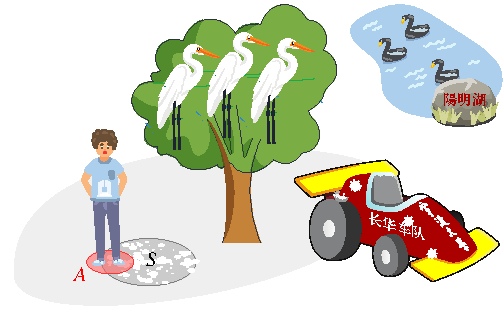
\includegraphics[width=\textwidth]{problem.pdf}
        \caption{鸟屎区域和人在地面投影区域的定义}\label{fig:problem}
    \end{minipage}
    \begin{minipage}[c]{0.075\textwidth}
         ~% 两图之间空点距离
    \end{minipage}
    \begin{minipage}[c]{0.45\textwidth}
        \centering
        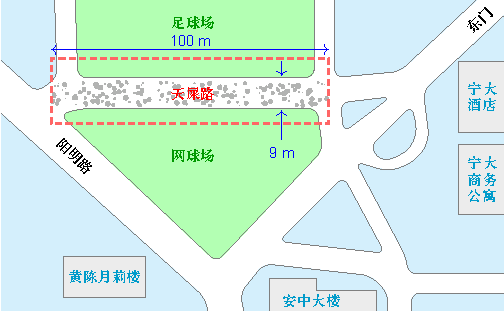
\includegraphics[width=\textwidth]{map.pdf}
        \caption{宁波大学其中一条天屎路示意图}
        \label{fig:map}
    \end{minipage}
\end{figure}


\section{表环境}
表格应具有三线表格式,因此常用 booktabs宏包,其标准格式如 \ref{tab:mytab} 所示。
\begin{table}[!htbp]
    \caption{标准三线表格}\label{tab:mytab} \centering
    \begin{tabular}{ccccc}
        \toprule[1.5pt]
        $D$(in) & $P_u$(lbs) & $u_u$(in) & $\beta$ & $G_f$(psi.in)\\
        \midrule[1pt]
        5 & 269.8 & 0.000674 & 1.79 & 0.04089\\
        10 & 421.0 & 0.001035 & 3.59 & 0.04089\\
        20 & 640.2 & 0.001565 & 7.18 & 0.04089\\
        \bottomrule[1.5pt]
    \end{tabular}
\end{table}

table 环境是一个将表格嵌入文本的浮动环境。tabular 环境的必选参数由每列对应一个格式字符所组成:\verb|c| 表示居中,\verb|l| 表示左对齐,\verb|r| 表示右对齐,其总个数应与表的列数相同。此外,\verb|@{文本}| 可以出现在任意两个上述的列格式之间,其中的文本将被插入每一行的同一位置。表格的各行以 \verb|\\| 分隔,同一行的各列则以\&分隔。 \verb|\toprule| 、\verb|\midrule| 和 \verb|\bottomrule| 三个命令是由booktabs宏包提供的,其中 \verb|\toprule| 和 \verb|\bottomrule| 分别用来绘制表格的第一条(表格最顶部)和第三条(表格最底部)水平线,\verb|\midrule| 用来绘制第二条(表头之下)水平线,且第一条和第三条水平线的线宽为 1.5pt,第二条水平线的线宽为 1pt 。引用方法与图片的相同。非三线表参考表 \ref{tab:Table-example}。
\begin{table}[!htb]
\centering
\caption{非三线表示例}\label{tab:Table-example}
\begin{tabular}{|c|c|c|c|c|}
\hline 
 & AAAAAA & BBBBBB & CCCCCC & DDDDDD\tabularnewline
\hline 
XXX & 1 & 2 & 3 & 4\tabularnewline
\hline 
YYY & 5 & 6 & 7 & 8\tabularnewline
\hline 
\end{tabular}
\end{table}

% %%%%%%%%%%%%%%%%%%%%%%%%%%%%%%%%%%%%%%%%%%%%%%%%%%%%%%%%%%%%%%%%%%%%%%%%%%%%


\chapter{参考文献与脚注}

\section{参考文献与引用}

参考文献对于一篇正式的论文来说是必不可少的,在建模中重要的参考文献当然应该列出。\LaTeX{}在这方面的功能也是十分强大的,下面进介绍一个比较简单的参考文献制作方法。有兴趣的可以学习 \verb|bibtex| 或 \verb|biblatex| 的使用。

这是一个简单的引用 \cite{zhangkun1994,zhukezhen1973},用 \verb|\cite{bibkey}| 来完成。如果不想上标,可用 \verb|\Cite{bibkey}| 实现(注意,"C"是大写),例如\Cite{scitor2000project}。


\section{脚注}

利用 \verb|\footnote{具体内容}| 可以生成脚注\footnote{脚注可以补充说明一些东西}。
